\documentclass[12pt,a4paper]{article}
\usepackage[utf8]{inputenc}
\usepackage[T1]{fontenc}
\usepackage[dutch]{babel}
\usepackage{amsmath}
\usepackage{amsfonts}
\usepackage{amssymb}
\usepackage{graphicx}
\usepackage{algpseudocode}
\usepackage{algorithm}
\usepackage{fullpage}
\usepackage{subfigure}


\author{Estelle Severs, Maarten Magits}
\title{Studentencursus TMI}
\begin{document}
	%TODO Screenshots van pseudocode vervangen door effectieve pseudocode. 
	\maketitle
	\tableofcontents
	\section*{Introductie}
	Toepassingen van de informatica (TMI) wordt ook wel Computationele geometrie (CG) genoemd.
	In het algemeen handelt dit domein over het berekenen en manipuleren van geometrische entiteiten/vormen en een oplossing te vinden voor geometrische problemen.
	Er vallen twee subdomeinen te onderscheiden:
	\begin{enumerate}
		\item \textbf{Combinatorial CG}: De studie van concrete objecten. Behandelt de discrete ruimte.
		\item \textbf{Numerical CG}: De studie van curves en functies. Eerder abstract.
	\end{enumerate}
	Dit OPO gaat grotendeels over de Combinatorial CG met slects een klein deeltje Numerical CG. In de slides volgen hier nog wat voorbeelden op, maar je kan ook gewoon de hoofdstukken beginnen bekijken voor goeie voorbeelden. 
	
	In deze cursus zullen we de volgende stappen telkens volgen voor het opmaken van een algoritme: 
	\begin{enumerate}
		\item Aanvankelijk negeren we de speciale gevallen. Op deze manier maken we een eerste versie van het algoritme
		\item Nu passen we ons algoritme aan op de speciale gevallen. Dit kan met (domme) if-then-else testen zullen we eerder vermijden. We willen het algoritme zo aanpassen zodat de speciale gevallen gewoon opgelost geraken. 
		\item Dan zal je het effectieve algoritme implementeren!
	\end{enumerate}
	
	
	\section{Convex Omhullende}
	Het deeltje over convex omhullende begint met wat basis definities over wat dit eigenlijk is. Er is daarna ook een figuur om het volledig duidelijk te maken. 
		\begin{description}
			\item[Convexe verzameling] Een vorm (shape) of verzameling (set) is convex indien voor elk paar punten die tot de verzameling behoren, het lijnsegment dat beide punten verbindt ook behoort tot die verzameling. 
			\item[Convex omhullende] Voor een deelverzameling van het vlak, is de convex omhullende de kleinst mogelijke convexe vorm die de hele deelverzameling bevat. 
		\end{description}
	Om je een idee te geven van het belang van zo een convex omhullende, geven we ook wat applicaties. Daarna zullen we ingaan op de algoritmes om ze te bepalen. 
		\begin{itemize}
			\item Als een verzameling punten staat voor een aantal obstakels, zal een robotarm het pad 	errond kiezen volgens de convex omhullende. 
			\item We kunnen bij het detecteren of twee figuren overlappen, de convex omhullende berekenen en dan zien of deze vormen al overlappen. Als dat niet het geval is, zullen de vormen zelf ook niet overlappen. 
			\item Om het puntenpaar te vinden dat het verst van elkaar gelegen is in een verzameling, is het relevant de convex omhullende te bepalen aanegzien alle punten die het verste van elkaar zitten in de verzameling ook op de convex omhullende zullen liggen. 
		\end{itemize}
	We gaan nu het bepalen van de convex omhullende bespreken. We gaan hier gebruik maken van een input aan punten \(P = {p_1, p_2, p_3, ..., p_n}\). De output zal de punten op de convexe veelhoek zijn geordend in klokwijzerzin. We zullen de convex omhullende noteren als $CH(P)$.
	
	
	\subsection{Brute Force algoritme}
	Het brute-force algoritme gaat voor elk paar aan punten nakijken of alle andere punten aan de rechterkant liggen. Als dit het geval is, is dit deel van de convexe veelhoek en wordt deze toegevoegd aan de lijst van edges E. De laatste stap zal er nog eens over de edges gegaan worden om deze in de juiste volgorde te steken. 
	De input is in dit geval een set punten P in een vlak. De output is dan een list $\mathcal{L}$ met de vertices van $CH(P)$ in wijzerzin. Hieronder is de pseudocode voor het algoritme
	\begin{figure}[h]
		\centering
		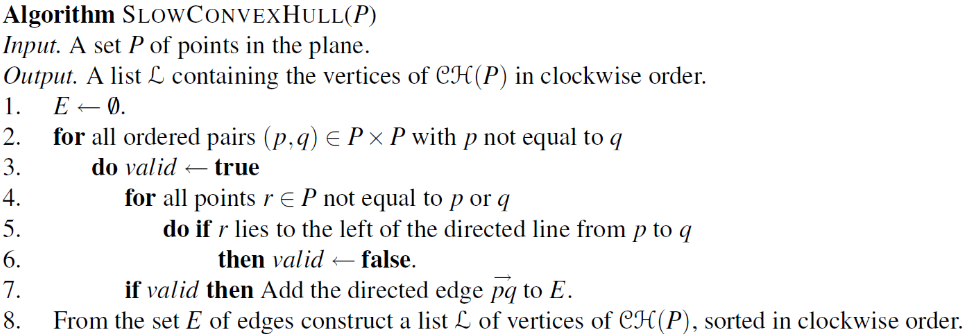
\includegraphics[width=0.9\linewidth]{afbeeldingen/slowconvexhull}
		\label{fig:slowconvexhull}
	\end{figure}
	
	De eerste lus zal $n^2$ keer lopen, gezien het voor elk paar hetgeen in de lus zal uitvoeren. In de lus zelf zal er nog eens over de punten gelopen worden om te kijken of deze allemaal rechts liggen van het gegeven punt, wat nog een $n$ keer zal lopen. De tijdscomplexiteit van dit algoritme is dus $O(n^3)$. 
	
	Naast het feit dat het algoritme helemaal niet efficiënt is, zijn er ook wat problemen in verband met de nauwkeurigheid van het berekenen of zo een punt links of rechts licht van een ander punt. Het kan zijn dat hierdoor punten fout worden bepaald terwijl ze wel links liggen van een edge. Een ander probleem is wanneer er meerdere punten op een lijn liggen, dit is dan een speciaal geval maar hier zou extra rekening mee gehouden moeten worden, het algoritme zal hier niet automatisch mee omgaan. Dit algoritme is dus duidelijk niet al te efficiënt en er zijn een paar gevallen waarbij het zelfs foute beslissingen kan maken. 
	
	
	\subsection{Incrementeel algoritme 	(Andrew's algorithm)}
	Dit algoritme zal de verzameling punten verdelen in een bovenhelft en in een onderhelft. Deze helften zullen dan in $O(n\log(n))$ volgens de x-as gesorteerd worden. Er zal dan volgens deze sortering gelopen worden om te kijken wanneer er tussen drie punten een 'rechterhoek' of een 'linkerhoek' wordt gemaakt. Als dit onduidelijk is, is hieronder een afbeelding met een voorbeeld waarom die hoeken uitmaken. 
	
	\begin{figure}[h]
		\centering
		\subfigure[]{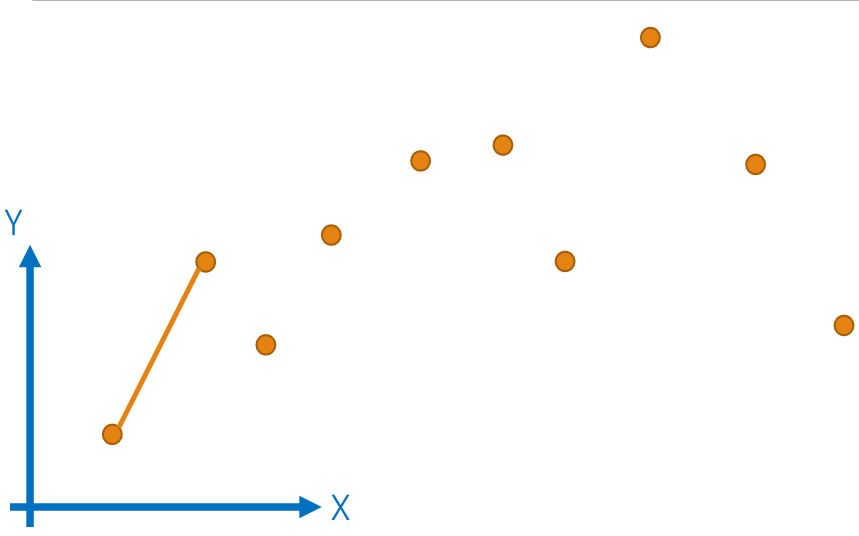
\includegraphics[width=0.24\textwidth]{afbeeldingen/first-convex}} 
		\subfigure[]{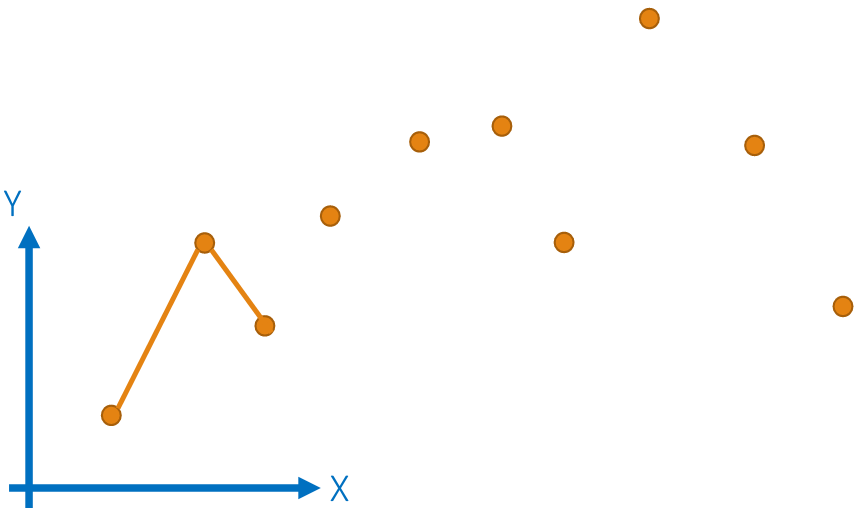
\includegraphics[width=0.24\textwidth]{afbeeldingen/second-convex}} 
		\subfigure[]{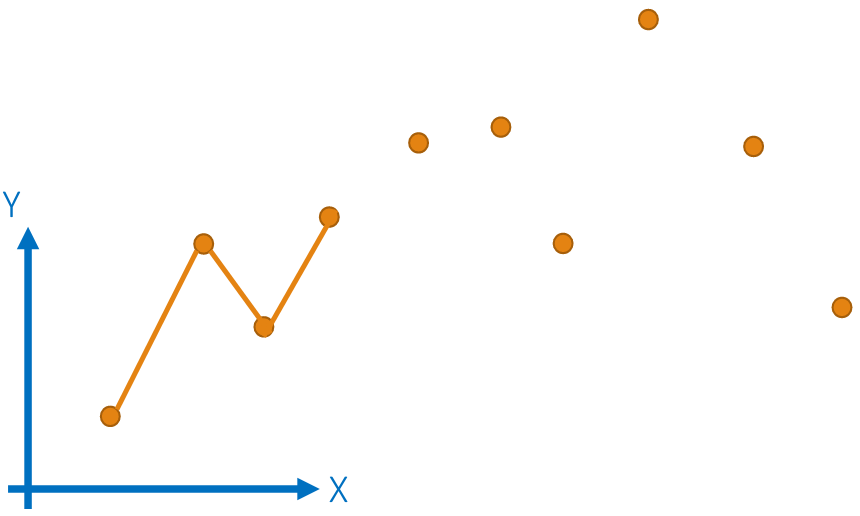
\includegraphics[width=0.24\textwidth]{afbeeldingen/third-convex}}
		\subfigure[]{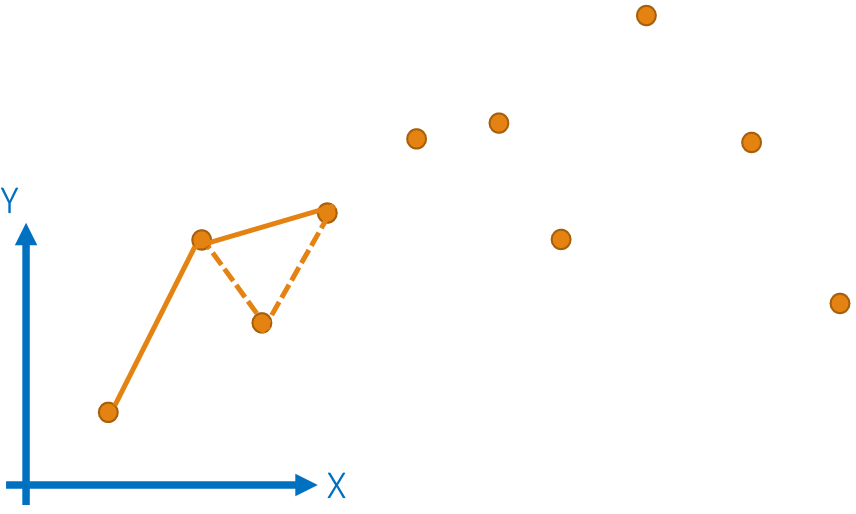
\includegraphics[width=0.24\textwidth]{afbeeldingen/fourth-convex}}
		\label{fig:incremental-example}
	\end{figure}
	Bij afbeelding c maken die punten duidelijk een linkerdraai, wat niet zou mogen voor een convex hull, dus zullen de twee edges verwijderd worden en vervangen worden door de nieuwe. Dit zal voor heel het puntenwolk verdergaan voor de bovenste helft. Voor duidelijkheid is hieronder nog de psuedocode
	\begin{figure}[h]
		\centering
		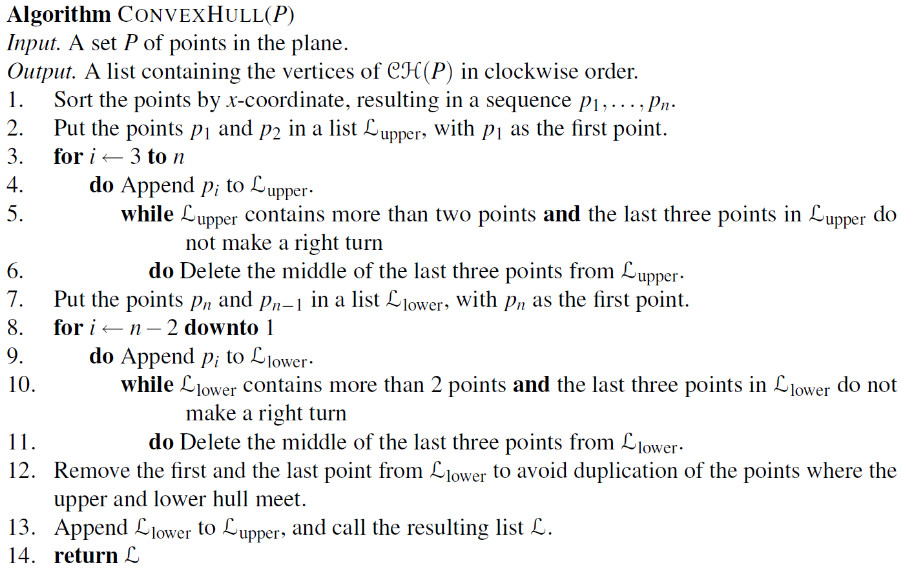
\includegraphics[width=0.9\linewidth]{afbeeldingen/convex-hull}
		\label{fig:convex-hull}
	\end{figure}

	De correctheid van het algoritme wordt bewezen d.m.v inductie: 
	\begin{itemize}
		\item Juiste bovengrens wordt berekend ${p_1, p_2}$
		\item Veronderstel dat we de juiste bovengrens berekend hebben voor ${p_1, p_2, ..., p_{i-1}}$
		\begin{itemize}
			\item $p_i$ toevoegen aan bovengrens - nieuwe bovengrens ligt boven de oude bovengrens
			\item Liggen alle punten ${p_1, p_2, ..., p_i}$ die niet behoren tot de bovengrens, beneden die bovengrens?
			\item Omwille van inductie tot $p_{i-1}$, kan enige mogelijkheid zijn dat een punt tussen $p_{i-1}$ en $p_i$ boven de bovengrens ligt, maar dit is onmogelijk, vermits we punten in gesorteerde volgorde behandelen. 
		\end{itemize}
	\end{itemize}
	Voor de tijdscomplexiteit weten we dat het sorteren van de punten $O(n\log(n))$ zal zijn terwijl voor de rest van het algoritme, we hoogstens één keer over elk punt zullen lopen, wat een tijdscomplexiteit geeft van $O(n)$. De totale tijdscomplexiteit van dit algoritme is dus \(O(n) + O(n\log(n)) = O(n\log(n))\).
	
	Ook voor dit algoritme zijn er speciale gevallen: wat als punten collineair zijn, wat met punten die hetzelfde x-coordinaat hebben en wat als er afrondingsfouten zijn in de hoeken. Dit kan allemaal opgelost worden met extra statements, maar dat geeft een lelijker algoritme. 
	
	
	\subsection{Graham's scan}
	Graham's scan zal niets aan het maken van de convex hull veranderen, maar zal het sorteren aanpassen. De punten zullen gesorteerd worden volgens poolhoek rond laagste meest linkse punt. Na het sorteren zullen de punten volgens de hoek overlopen worden om dan het verdere incrementeel algoritme toe te passen. De eerste van twee afbeeldingen bij Jarvis' march is een goede representatie van hoe de punten gesorteerd worden. 
	
	De tijdscomplexiteit is als volgt te bepalen. Het bepalen van het laagste punt is $O(n)$, het sorteren van de punten volgens punten zal $O(n\log(n))$ vragen en het overlopen zal zoals het vorige algoritme $O(n)$ vragen. De totale tijdscomplexiteit is dus $O(n\log(n))$. 
	
	
	\subsection{Jarvis's March}
	Jarvis' march zal beginnen zoals Graham's scan, beginnen met het uiterst links onderste punt en dan op poolhoeken sorteren, en zal die voor elk punt opnieuw doen. Dit wordt verduidelijkt door de onderstaande afbeeldingen; 
	
	\begin{figure}[h]
		\centering
		\subfigure[]{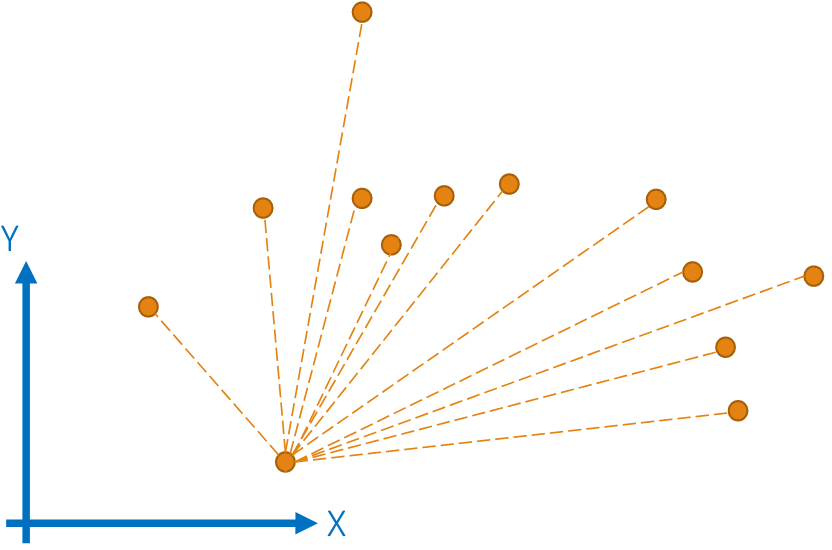
\includegraphics[width=0.45\textwidth]{afbeeldingen/first-jarvis}} 
		\subfigure[]{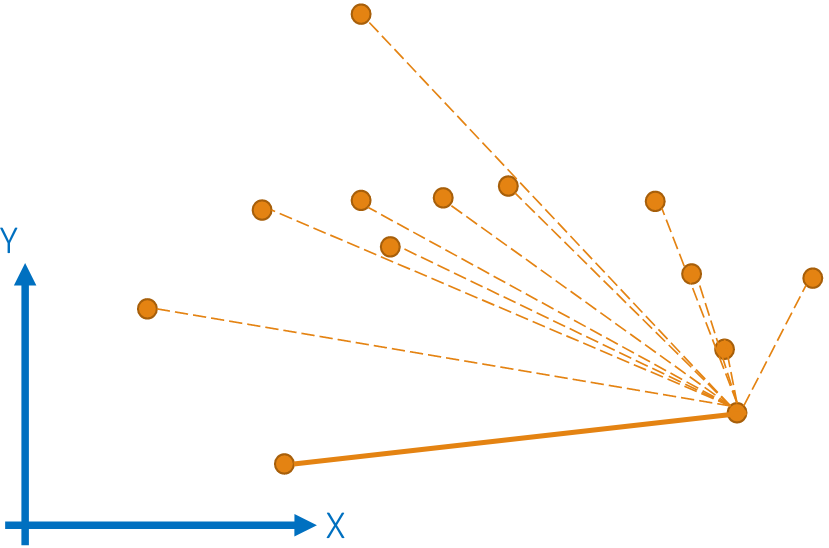
\includegraphics[width=0.45\textwidth]{afbeeldingen/second-jarvis}} 
		\label{fig:jarvis' example}
	\end{figure}

	Voor elk hoekpunt zal gekeken worden naar alle andere punten in de ruimte, hier voelen we aan dat in onze complexiteitsanalyse, we rekening zullen moeten houden met het aantal hoekpunten. Dit is het eerste algoritme waarbij we rekening houden met de output, wat resulteert in een \textit{output-afhankelijke tijdscomplexiteit}. Het aantal hoekpunten en dus het aantal elementen in de output zal in de tijdscomplexiteit $h$ zijn. Gezien we voor elk hoekpunt ongeveer alle andere punten moet overlopen, is de tijdscomplexiteit $O(n\cdot h)$.
	
	Dit algoritme zal dus bijna lineaire tijd hebben bij heel weinig hoekpunten, wat veel beter is dan graham's scan. Anderzijds kan het bijna een kwadratische tijdscomplexiteit worden als het aantal hoekpunten even groot wordt als het algemeen aantal punten. 
	
	Jarvis' march zal bij een klein aantal hoekpunten het logisch algoritme zijn terwijl graham's scan beter is voor een groter aantal. 
	
	%TODO navragen!
	

	\subsection{Verdeel-en-heers}
	Dit is een strategie die we al hebben zien terugkeren bij sorteeralgoritmes. We splitsen het probleem op, we lossen de kleinere problemen op en dan combineren we de oplossingen. De recursie stopt als de verzameling triviaal klein wordt. De tijdscomplexiteit van zo'n algoritmes is vaak $O(n\log(n))$. 
	
	Een manier is om de puntenwolk telkens willekeurig te verdelen en dan de twee convex omhullenden telkens te mergen op de meest extreme punten. Dit lijkt al heel goed, maar willekeurig kan ook heel slechte algoritmes brengen, dus is dit niet altijd het meest ideale. 
	
	Een tweede manier is om de puntenwolk telkens perfect in twee te verdelen volgens de x-coördinaten. De merge-operatie is dan telkens een bovenraaklijn en een onderraaklijn zoeken om deze te verbinden en nog steeds een convex omuhllende te verkrijgen. Deze onder- en bovenbrug is niet altijd het onderste en/of bovenste punt van een puntenwolk, hier bestaat dus een algoritme voor: 
	
	\begin{figure}[h]
		\centering
		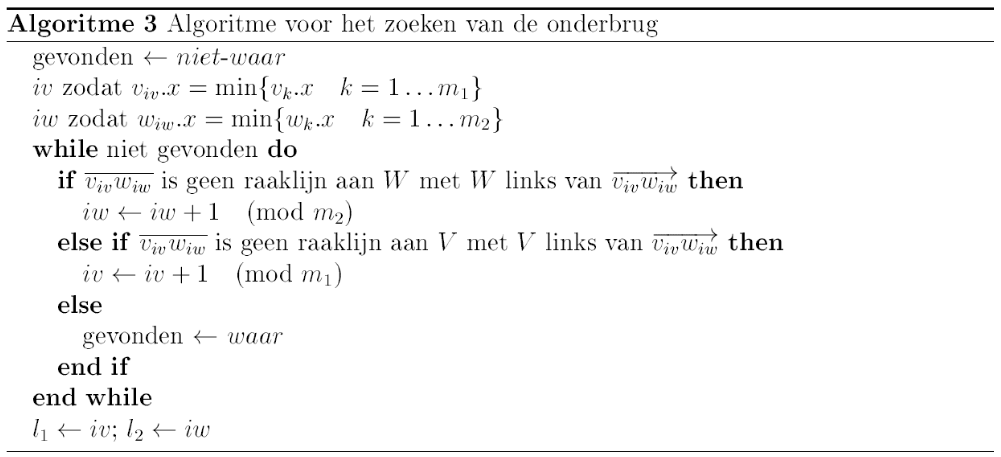
\includegraphics[width=0.9\linewidth]{afbeeldingen/verdeel-en-heers-convex}
		\label{fig:verdeel-en-heers-convex}
	\end{figure}
	%TODO verdere uitleg zoeken want hier zou mondelinge uitleg best ook bijkomen
	
	%TODO Typische examenvragen nog op te lossen
	\subsection{Typische examenvragen}
	\begin{itemize}
		\item \textbf{Leg het Graham Scan algoritme uit voor de berekening van een convex omhullende veelhoek ven een set punten:}\\
		\item \textbf{Hoe zou je Graham's Scan en Jarvis' March met elkaar vergelijken? Wat zijn sterke en zwakke punten van beide algoritmen?:}\\
		\item \textbf{Stel dat je een verzameling punten hebt, waarvan een deel punten  colineair zijn (ttz op dezelfde lijn liggen). Welke problemen zou je kunnen ontmoeten bij het Graham's Scan algoritme? Bij Jarvis' March?:}\\
		\item \textbf{Stel dat je de convex omhullende wil berekenen van een set van n lijnsegmenten. Hoe zou je dit aanpakken?:}\\
		\item \textbf{Zou je het verdeel-en-heers algoritme ook kunnen toepassen als je de verzameling punten in 4 verdeelt - bijvoorbeeld zowel via de x-mediaan als de y-mediaan? Op welke manier kan je dan 4 convex omhullende veelhoeken combineren tot 1 veelhoek?:}\\
		\item \textbf{Bij het verdeel-en-heers algoritme kan je zowel een verdeling van de x-mediaan als volgens de y-mediaan toepassen. Op alle recursieve niveau's zou je telkens een andere beslissing kunnen nemen (verdelen volgens x of y). Van welke factoren zou deze keuze kunnen afhangen?:}\\
		\item \textbf{In welke mate is algoritme *vul hier een convex omhullende algoritme in * bestand tegen kleine rekenfouten? Levert het algoritme telkens een gesloten veelhoek? Soms zelfs geen veelhoek? Een concave veelhoek? Wat zijn mogelijke oorzaken van dergelijke fouten?:}\\
	\end{itemize}


	\section{Intersecties van lijnstukken}
	In dit hoofdstuk worden algoritmes besproken om snijpunten tussen lijnstukken te vinden. 
	\subsection{Brute Force algoritme}
	Het brute force algoritme zal domweg, zoals wel verwacht, elk lijnstuk met elk ander evalueren op een snijpunt. De pseudocode ervoor is hier te vinden:
	\begin{figure}[h]
		\centering
		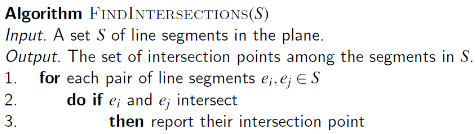
\includegraphics[width=0.8\linewidth]{afbeeldingen/find-Intersections}
		\label{fig:find-intersections}
	\end{figure}
	Het is duidelijk dat de tijdscomplexiteit van dit algoritme dus altijd $O(n^2)$ zal zijn en dat dit een \textit{input-afhankelijke} complexiteit heeft. Wanneer elk lijnstuk met elkaar snijdt kan dit geen kwaad, maar als geen enkel lijnstuke met een ander snijdt, zal je hier heel veel tijd mee verliezen. 
	
	
	\subsection{Doorlooplijn algoritme}
	%TODO stel u voor, ge weet ondertussen nog niet wat een doorlooplijn is
	Een doorlooplijn is een denkbeeldige lijn die door de dataset loopt en bijhoudt welke lijnsegmenten actief zijn en dus potentieel elkaar kunnen snijden. Als twee lijnsegemnten op die lijn zitten kan het zijn dat ze elkaar snijden, als ze niet op een moment gelijktijdig op de lijn zitten, is er geen kans dat ze elkaar snijden en moeten ze dus niet geëvalueerd worden op snijpunten. Als eerste zullen de punten dus gesorteerd moeten worden op de y-as volgens de begin- en eindpunten van de lijnsegmenten. Deze zouden dan terechtkomen in een event queue om deze af te lopen en bij elk punt een actie te ondernemen. Bij een startpunt worden alle actieve lijnsegemten geëvalueerd met het nieuwe toegevoegde lijnsegmenten om snijpunten te zoeken. Zo wordt een deel van de lijnsegmenten gefilterd en is het geen bruteforce. De datastructuur voor de doorlooplijn zou in dit geval gewoon een lijst kunnen zijn aangezien deze niet gesorteerd hoeven te zijn. 
	
	De worst case van dit algoritme is wanneer er allemaal lijnstukken parallel verticaal naast elkaar liggen. Dan wordt elk lijnstuk met elkaar vergeleken ondanks dat we een doorlooplijn gebruiken en is het even onefficiënt als een brute force algoritme. 
		
	\subsection{Doorlooplijn++}
	In de verbeterde doorlooplijn zullen we niet naar alle actieve lijnstukken kijken op de lijn, maar enkel naar de buren van het toegevoegde lijnstuk. Nu zal er dus wel een datastructuur nodig zijn om deze sortering bij te houden, dit zal het beste gaan met een gebalanceerde zoekboom. Er zijn verschillende soorten 'events' in dit algoritme, je kan van elk een voorbeeld zien in de onderstaande afbeelding.  
	
	\begin{figure}[h]
		\centering
		\subfigure[]{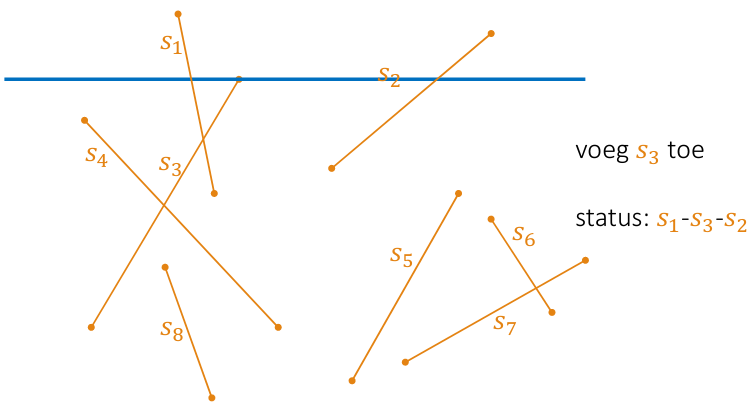
\includegraphics[width=0.24\textwidth]{afbeeldingen/first-doorlooplijn}} 
		\subfigure[]{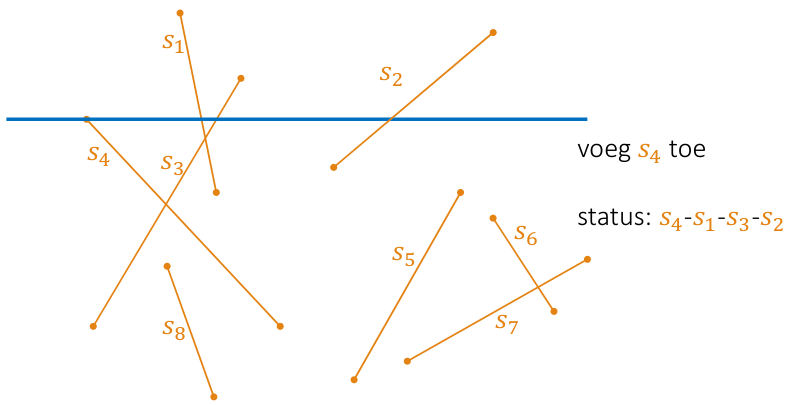
\includegraphics[width=0.24\textwidth]{afbeeldingen/second-doorlooplijn}} 
		\subfigure[]{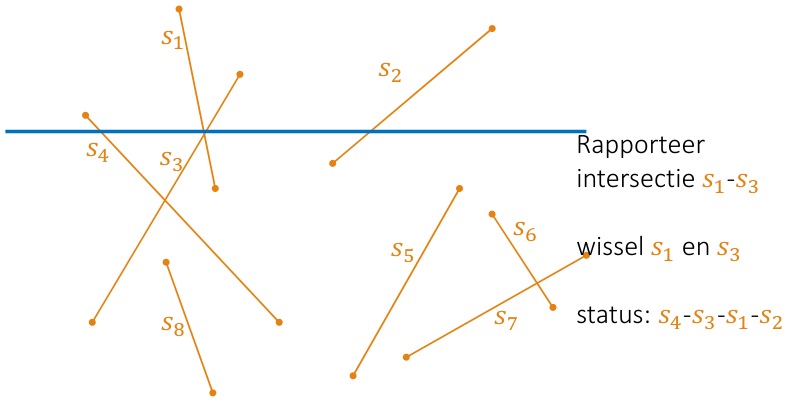
\includegraphics[width=0.24\textwidth]{afbeeldingen/third-doorlooplijn}}
		\subfigure[]{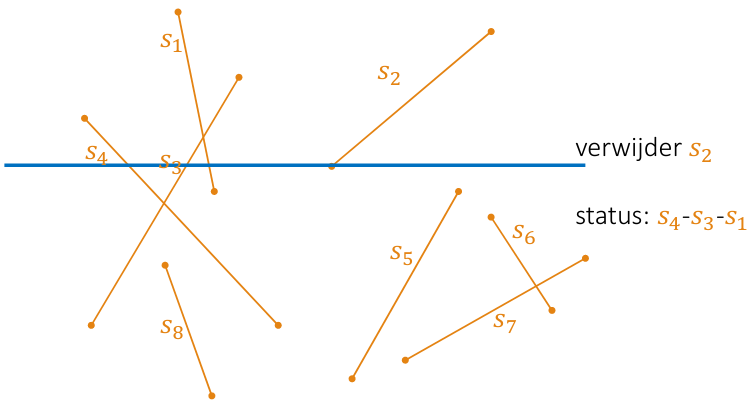
\includegraphics[width=0.24\textwidth]{afbeeldingen/fourth-doorlooplijn}}
		\label{fig:sweepline-example}
	\end{figure}

	De event queue zal in dit geval ook een gebalanceerde zoekboom zijn, het is geen priority queue aangezien er niets is dat een 'prioriteit' heeft.
	\begin{description}
		\item[Start event:] Een start event is wanneer een nieuw lijnstuk actief wordt op de doorlooplijn, in dat geval zal het nieuwe lijnstuk vergeleken worden met zijn buren op snijpunten. Als er snijpunten worden gevonden, worden deze toegevoegd aan de event queue. 
		\item[intersectoin event:] Bij een snijpunt zal het algoritme de volgorde van de lijnstukken op de status queue verwisselen en deze lijnstukken zullen dan met hun nieuwe buren vergeleken worden voor nieuwe snijpunten. 
		\item[End event:] Het einde van een lijnstuk betekent dat dit lijnstuk van de status queue gehaald moet worden en dat er moet gekeken worden of de nieuwe buren elkaar snijden. 
	\end{description}

	De pseudocode is hieronder te vinden: 
	
	\begin{figure}[h]
		\centering
		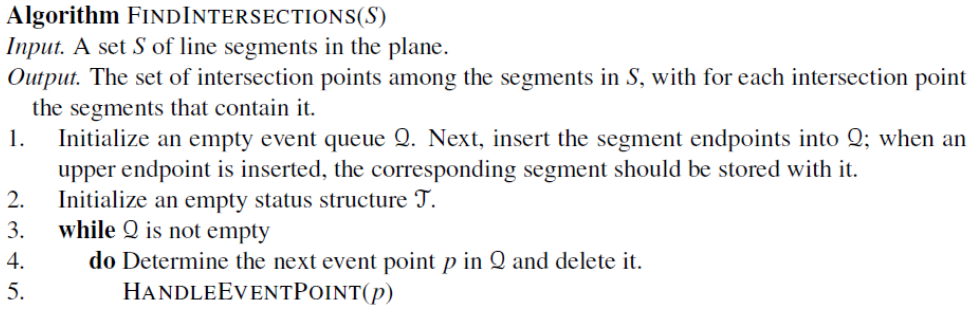
\includegraphics[width=0.9\linewidth]{afbeeldingen/find-intersections++}
		\label{fig:find-intersections++}
	\end{figure}
	
	De correctheid van dit algoritme wordt als volgt bewezen: Indien twee lijnsegmenten elkaar snijden, moet er ergens een event zijn boven het intersectiepunt, waar beide lijnsegmenten elkaars buren worden.\\
	Indien de doorlooplijn zich net boven een intersectiepunt p bevindt, zijn $s_i$ en $s_j$ aangrenzend (en worden dus getest op intersectie).\\
	Initieel is de status leeg, er moet dus ergens een event zijn dat $s_i$ en $s_j$ aangrenzend maakt.
	
	Elk event is begrensd door een tijdscomplexiteit van $O(\log(n))$. De lus zal 2n + k keer uitgevoerd worden, met $n$ het aantal cirkels en $k$ het aantal snijpunten. De lus zal dus  $O(n + k)$ overlopen worden, wat een totaal geeft van $O((n+k)\log(n))$. Qua geheugen zal de status vast zijn door het maximaal aantal elementen dat er op de lijn tevoorschijn kan komen, wat dus $O(n)$ is. De event queue zal begrensd zijn door $2n + k$ events, wat in het ergste geval kan uitkomen op $O(n^2)$. 
	
	Een speciaal geval kan twee punten zijn die dezelfde y-waarde hebben, dan kan de event queue het niet juist sorteren. Dit kan opgelost worden door de doorlooplijn zogezegd wat schijner te laten lopen. Een ander probleem is het samenvallen van events (het einde van een lijnstuk is gelijk aan het begin van een ander lijnstuk.) Hier moeten dan tijdens het implementeren bepaalde keuzes gemaakt worden, maar dit kan ook opgelost worden. %TODO moet hier nog iets bij? 


	\subsection{Doubly-connected edge list}
	Een DCEL is een manier om een oppervlak met lijnen in een datastructuur te steken en zo gemakkelijk over de datastructuur kunnen verplaatsen. Eerst volgen wat termen die belangrijk zijn om te kunnen praten over deze DCEL. 
	
	\begin{figure}[H]
		\centering
		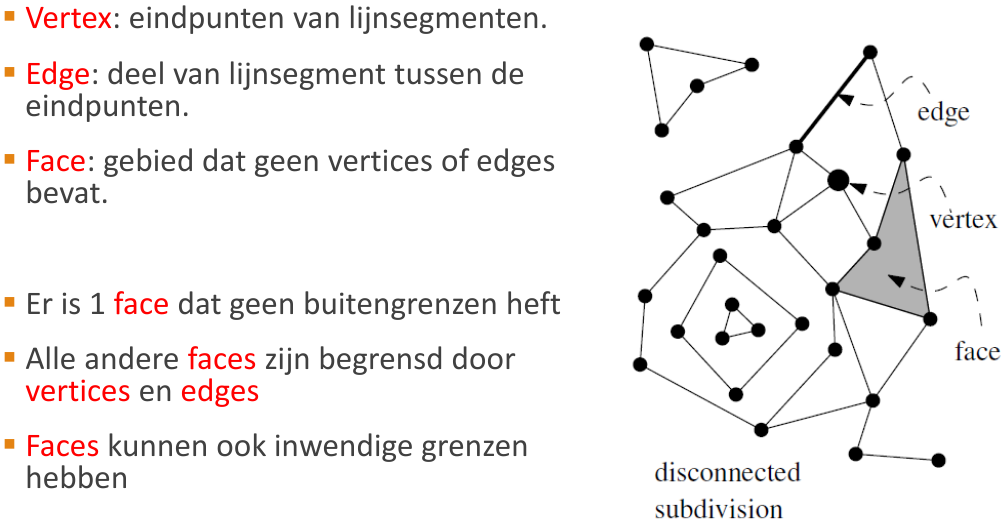
\includegraphics[width=0.8\linewidth]{afbeeldingen/DCEL-termen}
		\label{fig:dcel-termen}
	\end{figure}

	Het centrale idee is dat elke edge uit bovenstaande afbeelding kan gemaakt worden uit 2 'half-edges'. Deze half edges hebben elk een oorsprong-vertex, een twin (de andere half edge), een incidentface (face aan de linkerkant van de half-edge), een next en een prev. Elke vertex bestaat uit coördinaten en een incidentEdge (de edge startende in de vertex). 
	
	Met deze datastructuur kunnen we gemakkelijker de overlay van twee vlakverdelingen bepalen. Dit is eignelijk aanvankelijk het construeren van een DCEL uit twee DCEL's, wat door een doorloopalgoritme zal gebeuren. Ook hier werken we met events: 
	\begin{itemize}
		\item Een vertex van S1
		\item Een vertex van S2
		\item Een intersectiepunt van een edge van S1 met een edge van S2. 
		\begin{figure}[H]
			\centering
			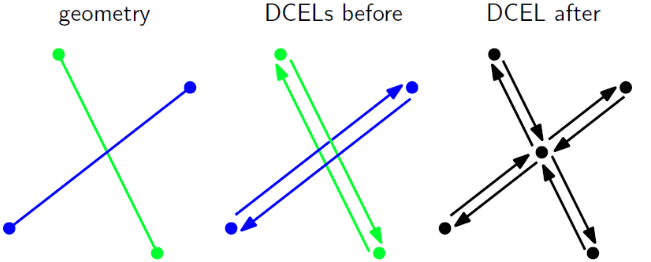
\includegraphics[width=0.7\linewidth]{afbeeldingen/intersection-DCEL}
			\label{fig:intersection-dcel}
		\end{figure}
		\item De edge van S1 snijdt met een vertex van S2 (of omgekeerd)
		\begin{figure}[H]
			\centering
			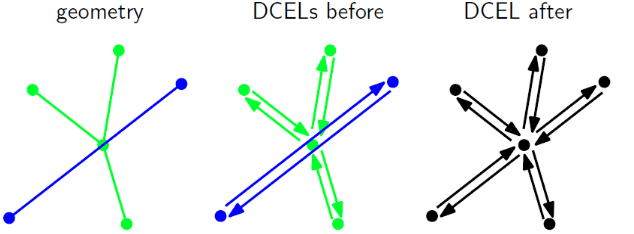
\includegraphics[width=0.7\linewidth]{afbeeldingen/DCEL-vertex&edge}
			\label{fig:dcel-vertexedge}
		\end{figure}
		\item Samenvallende vertices van S1 en S2
		\begin{figure}[H]
			\centering
			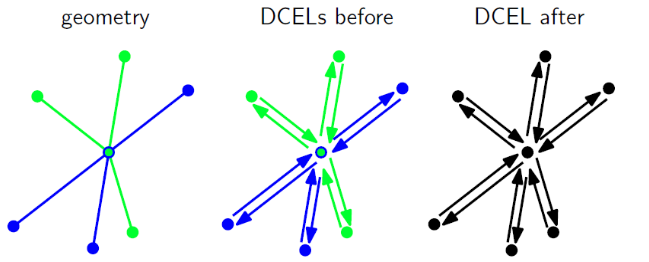
\includegraphics[width=0.7\linewidth]{afbeeldingen/DCEL-vertices}
			\label{fig:dcel-vertices}
		\end{figure}
	\end{itemize}

	Om de faces te bepalen, zal de nieuwe DCEL overlopen moeten worden om alle loops te detecteren en de inwendige en uitwendige grenzen te bepalen. Een face moet dan geconstrueerd worden voor elke uitwendige grens (+ het buitengebied). Van de inwendige grenzen kunnen we het meest links punt bepalen (van de vorm) en zodra een andere edge is gevonden, wordt deze vorm overlopen. Dit is dan de vorm waarbinnen de aanvankelijke vorm ligt. Dan kan een structuur zoals hieronder gemaakt worden. Deze indelingen zijn gemakkelijk om booleaanse opdrachten te gebruiken op veelhoeken.
	
	\begin{figure}[H]
		\centering
		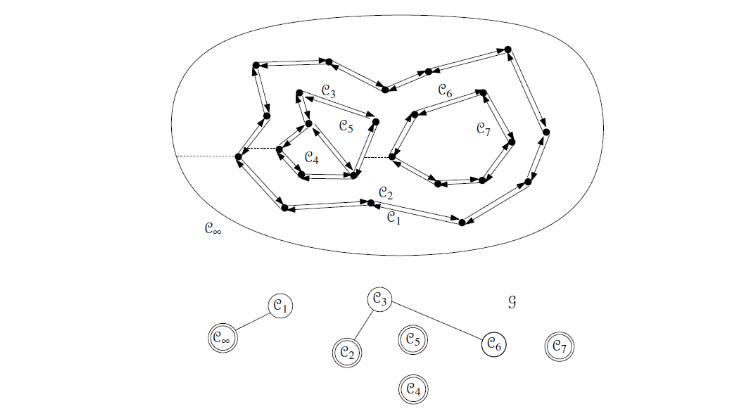
\includegraphics[width=0.7\linewidth]{afbeeldingen/DCEL-faces}
		\label{fig:dcel-faces}
	\end{figure}
	
	Voor de tijdscomplexiteit is de volgende afbeelding het bewijs (cuz ja, ik ben effe lui):
	
	\begin{figure}[H]
		\centering
		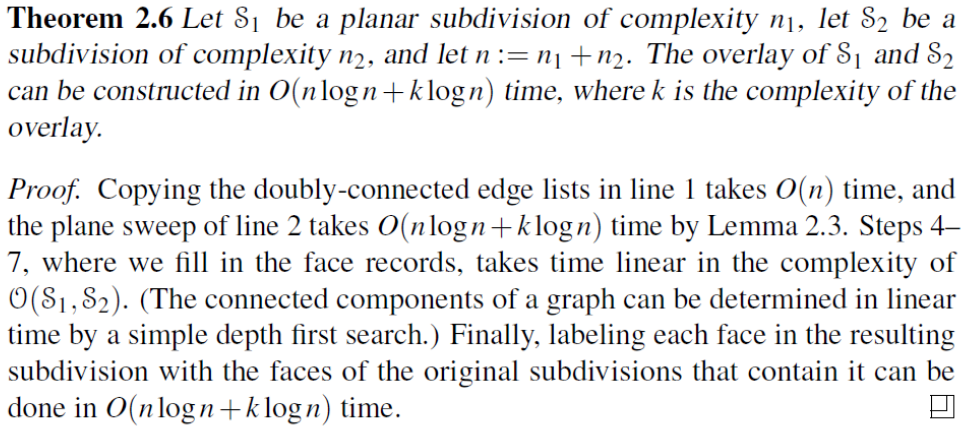
\includegraphics[width=0.7\linewidth]{afbeeldingen/DCEL-bewijs}
		\label{fig:dcel-bewijs}
	\end{figure}
	
	
	\subsection{Typische examenvragen}
	\begin{itemize}
		\item \textbf{Wat is de algemene idee van sweep-line algoritmen?:}\\
		\item \textbf{Beschrijf het algoritme om alle intersectiepunten in een verzameling lijnstukken te vinden. Bespreek ook de tijdscomplexiteit:}\\
		\item \textbf{Bespreek de Double-Connected-Edge-List als datatstructuur. Wat zijn voor- en nadelen van deze datastructuur?:}\\
		\item \textbf{Bespreek welke operaties er precies moeten gebeuren bij de afhandeling van <event van type X> bij het berekenen van de overlay van 2 vlakindelingen:}\\
	\end{itemize}
	
	
	\section{Triangulaties van veelhoeken}
	Dit deel begint met een klein voorbeeld als context. Stel dat je in een museum werkt en moet besluiten waar de bewakers 's nachts zullen staan. Je wilt natuurlijk zo min mogelijk (stilstaande) bewakers voor de ruimte die je moet bewaken. Dit wordt het \textit{Museumprobleem} genoemd. Bij deze probleemstelling komen dan ook de vraag: Wat is het minimaal aantal bewakers dat nodig is voor een n-hoek? Hier wordt dan ook een max over min forumlering gebruikt: Wat is het grootste aantal bewakers dat een veelhoek minimum nodig heeft? Je kan een 12-hoek bijvoorbeeld opdelen met 1 bewaker en met 4 bewakers, het maximum van de minima is hier 4 en dat is wat we dan zoeken. Dit getal schrijven we als $G(n)$ met n het aantal hoeken. Wat vanzelfsprekend is, is dat $G(n) \geq 1$ en dat $G(n) \leq n$ maar dit is te algemeen, we moeten specifieker gaan zoeken. Na een aantal voorbeelden is het duidelijk dat dit getal gelijk is aan $\lfloor n/3\rfloor$. Dit is dus het aantal bewakers dat voor een veelhoek met n hoeken altijd genoeg zal zijn om heel de ruimte te bewaken. 
	
	\subsection{Triangulaties}
	Een triangulatie is het toevoegen van zo veel mogelijk niet snijdende diagonalen in de veelhoek. Een diagonaal is een lijnstuk tussen twee hoekpunten die strikt zichtbaar zijn tegenover elkaar. Zoals je wel al merkt is zo een triangulatie niet uniek, er bestaan er heel veel en er is niet één juiste. Wat we met zekerheid kunnen zeggen is dat elke veelhoek kan getrianguleer worden om uit te komen op $n-2$ driehoeken. We bewijzen die door middel van inductie: 
	- $n-3$ : triviaal (1 driehoek wordt getrianguleerd in 1 driehoek).\\
	- $n > 3$ : 
	\begin{itemize}
		\item We construeren een diagonaal in $P$:
		\begin{itemize}
			\item $v$ is meest linkse vertex van $P$, met buren $u$ en $w$
			\item Geval 1: Indien $\overline{uw}$ binnen $P$ ligt $\rightarrow$ $\overline{uw}$ is een diagonaal
			\item Geval 2: er liggen vertices van $P$ binnen de driehoek $\vartriangle uw$:
			
			neem $v'$ als verst verwijderde van de lijn $\overline{uw}$. $\overline{vv'}$ kan $P$ niet snijden $\rightarrow$ $\overline{vv'}$ is een diagonaal. 
		\end{itemize}
		\item De diagonaal verdeelt $P$ in $P_1$ en $P_2$, met $m_1$ en $m_2$ vertices
		\item (veronderstel dat de stelling geldt voor $m<n)$
		\begin{itemize}
			\item $P_1$: $m_1$ vertices, triangulatie in $m_1$-2 driehoeken. 
			\item $P_2$: $m_2$ vertices, triangulatie in $m_2$-2 driehoeken. 
			\item $m_1 - m_2 = n+2$
		\end{itemize}
		\item $\rightarrow$ Triangulatie van $P$ telt $(m_1 -2) + (m_2 - 2) = n-2$ driehoeken. 
	\end{itemize}
	In het museumprobleem kunnen we gebruik maken van deze triangulatie: 
	\begin{figure}[H]
		\centering
		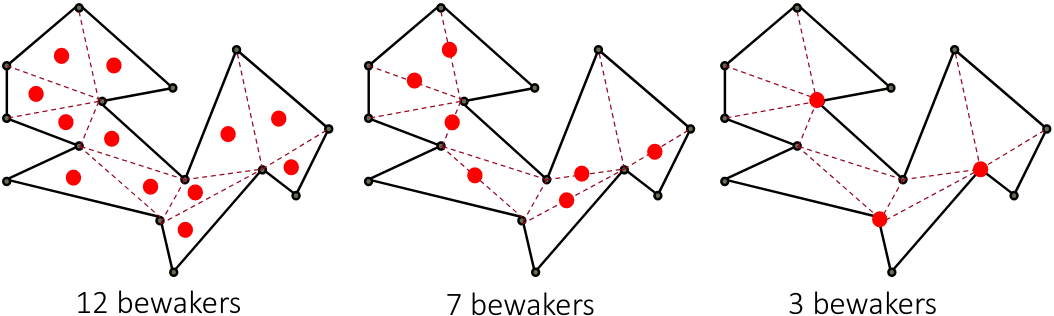
\includegraphics[width=0.9\linewidth]{afbeeldingen/triangulatie-bewakers}
		\label{fig:triangulatie-bewakers}
	\end{figure}
	Het is duidelijk dat de laatste figuue zorgt voor een optimale oplossing: zo weinig mogelijk bewakers die nog steesd de volledige ruimte in het oog kunnen houden. Het vinden van deze perfecte plekken kan aan de hand van een 'kleuring'. 
	
	
	\subsection{kleuring}
	Een kleuring is het toekennen van kleuren aan vertices zodat verbonden vertices een verschillende kleur hebben. Voor onze situatie gebruiken we een 3-kleuring, elke vertex mag dus een van die drie kleuren hebben. Zo en kleurring kan gemakkelijk gevonden worden door telkens een driehoek te halen uit de triangulatie, elke keer als die driehoek terug toegevoegd moet worden zal de nieuwe hoek die nog geen kleurring heeft, eenduidig bepaald een van de drie kleuren bevatten. Na het kleuren van de vertices kan je dan besluiten een van de kleuren te kiezen om dan de bewakers daar te positioneren. Het is ergens wel logisch dat er van sommige kleuren meer zijn dan anderen, net zoals hiernoder te zien is. 
	\begin{figure}[h]
		\centering
		\subfigure[]{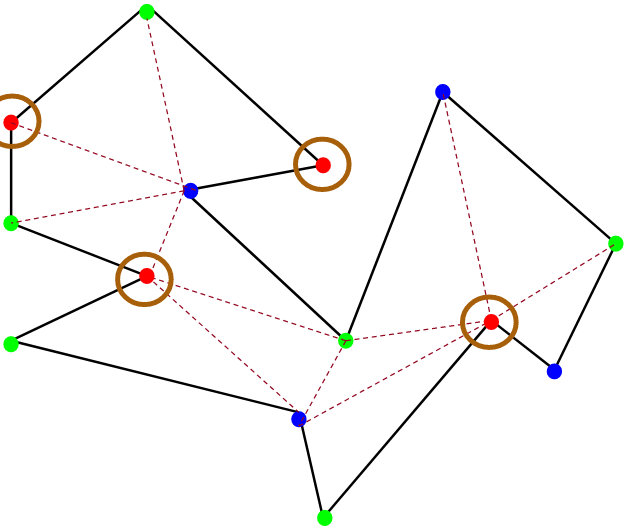
\includegraphics[width=0.32\textwidth]{afbeeldingen/triangulatie-rood}} 
		\subfigure[]{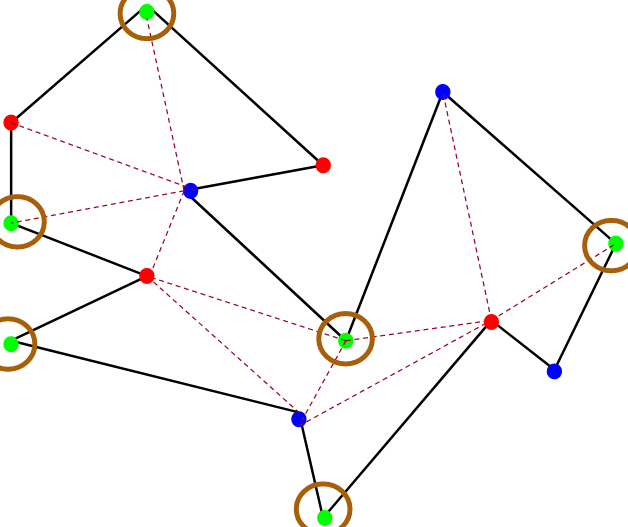
\includegraphics[width=0.32\textwidth]{afbeeldingen/triangulatie-groen}} 
		\subfigure[]{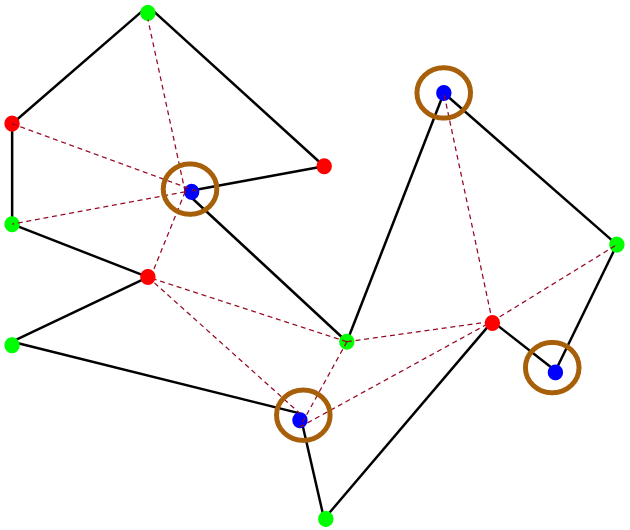
\includegraphics[width=0.32\textwidth]{afbeeldingen/triangulatie-blauw}}
		\label{fig:trianuglation-colours}
	\end{figure}
	Het is hier duidelijk dat rood en blauw elk een goeie verdeling hebben, maar ook niet allebei optimaal. Bij beiden zou er nog een bewaker kunnen wegvallen en zou heel het oppervlak nog steeds bewaakt zijn. Gezien dit een 3-kleuring is, wordt elke kleur maximaal $n/3$ keer gebruikt en vermits $n$ geheel is: $\lfloor n/3 \rfloor$. Een goede voorstelling hiervan is ook Chvátal's kam. 
	\begin{figure}[H]
		\centering
		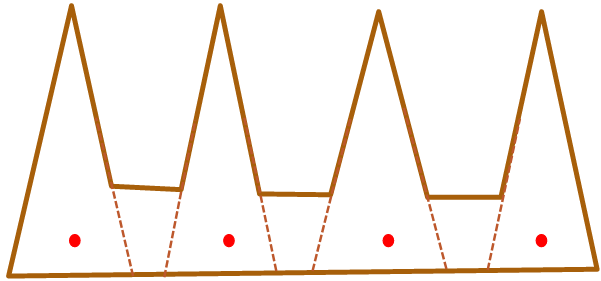
\includegraphics[width=0.6\linewidth]{afbeeldingen/triangulatie-kam}
		\label{fig:triangulatie-kam}
	\end{figure}

	Het is duidelijk dat dit het ergste geval is. We weten nu de theorie achter deze triangulaties, maar we moeten nog ontdekken hoe we deze moeten opstellen. 
	
	
	\subsection{Hoe te trianguleren}
	Het trianguleren begint best door elke keer een oor af te snijden en zo verder te zoeken naar een triangulatie binnen de nieuwe veelhoek met $n-1$ vertices. De tijdscomplexiteit van die algoritme zou dan $O(n^2)$ zijn. Voor convexe veelhoeken wordt die zelfs $O(n)$. 
	
	Om een veelhoek te trianguleren beginnen we eerst met het definiëren van een 'y-monotone' veelhoek. Een veelhoek is y-monotoon als een horizontale lijn de veelhoek over slechts één interval snijdt. De veelhoek wordt opgesplitst in y-monotone veelhoeken en van elk van deze veelhoeken wordt dan de triangulatie gezocht. In een veelhoek kan elke hoek ingedeeld worden als volgt: 
	\begin{figure}[H]
		\centering
		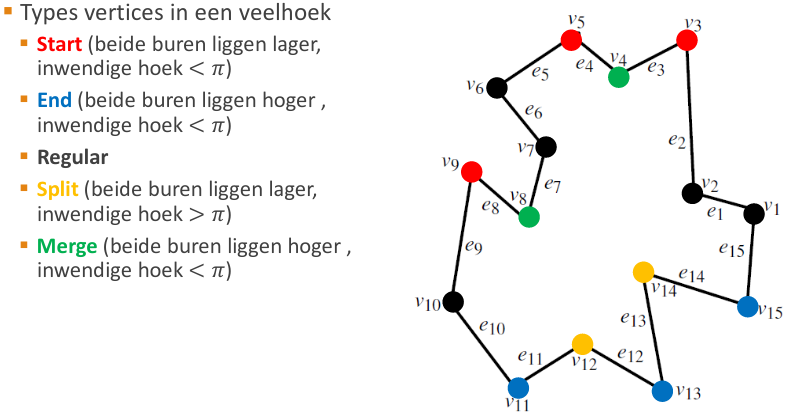
\includegraphics[width=0.7\linewidth]{afbeeldingen/triangulaties-y-monotoon}
		\label{fig:triangulaties-y-monotoon}
	\end{figure}
	Het is relatief duidelijk dat de split en merge knopen het probleem vormen om de veelhoek y-monotoon te maken. Wanneer een veelhoek niet y-monotoon is, is het duidelijk dat het of een split node heeft, of een merge node, deze zullen we moeten wegwerken met een algoritme. Het algoritme zal dan een diagonaal maken bij merge-vertices die naar beneden gaat, en bij split-vertices die naar boven gaat. Dit zal, you guessed it, met een doorlooplijn algoritme gebeuren. Hierij initialiseren we een helper voor een edge, deze helper is de laatste vertex boven de doorlooplijn, waarbij de horizontale tussen de edge en de vertex volledig binnen de veelhoek ligt. 
	
	Om een merge vertex juist op te lossen, kijk je telkens er een nieuwe helper wordt geïnitialiseerd, of de oude helper een merge vertex is. Als die een merge vertex is, dan zal de oude en de nieuwe helper verbonden worden. Een split vertex zal gelijkaardig opgelost worden, maar dan zal de split een nieuwe helper zijn en wordt deze verboncen met de oude helper. Dit algoritme kan gebeuren in $O(n\log(n))$ met het geheugen in lineaire tijd. 
	
	De triangulatie van de overbleven monotone veelhoeken kan dan gedaan worden met een greedy algoritme. We sorteren de vertices volgens y-coördinaat en zetten de twee eerste vertices op de stack. Daarna wordt er zo veel mogelijk getrianguleerd naar wat er op de stack staat. Dit geldt voor alle geldige diagonalen op de stack. Zodra er een ongeldige diagonaal is, wordt er naar de laatste vertex gekeken en van daar uit nieuwe diagonalen maken. Hier is een goede illustratie van in de slides. 
	
	Dit algoritme werkt in lineaire tijd $\rightarrow$ $O(n)$. Met het algoritme om de veelhoek in te delen in monotone veelhoeken zal de totale complexiteit $O(n\log(n))$ zijn. 
	
	
	\subsection{Typische examenvragen}
	\begin{itemize}
		\item \textbf{Bewijs dat een oplossing voor het “museumprobleem” of “art gallery problem” voor een (eenvoudige) veelhoek met n hoeken een bovengrens heeft gelijk aan  n/3 (naar beneden afgerond) bewakers:}\\
		\item \textbf{Stel dat we een klasse (eenvoudige) veelhoeken hebben, met als eigenschap dat ze d.m.v. niet-snijdende diagonalen in de veelhoek steeds kunnen opgesplitst worden in een verzameling convexe vierhoeken. Welke uitspraken kan je doen i.v.m. het “museumprobleem” of “art gallery problem” voor deze klasse van veelhoeken?:}\\
		\item \textbf{Bewijs dat elke eenvoudige veelhoek met n hoekpunten kan getrianguleerd worden in n-2 driehoeken. Geef duidelijk alle stappen in de redenering:}\\
		\item \textbf{Op welke manier kunnen we een veelhoek splitsen in een aantal monotone veelhoeken?:}\\
		\item \textbf{In het globale algoritme om een veelhoek te trianguleren splitsen we eerst de veelhoek op in y-monotone veelhoeken. Maakt het een verschil voor de finale triangulatie als we zouden splitsen in x-monotone driehoeken?:}\\
	\end{itemize}
	
	
	\section{Lineaire programming \& gerandomiseerde algoritmen}
	De probleemstelling van het eerste deel van dit stuk is: Kan een bepaald ontwerp gemaakt worden met één enkele gietvorm en kan dat object in één vloeiende beweging verwijderd worden. De probeemstelling is gevisualiseerd als volgt: 
	\begin{figure}[H]
		\centering
		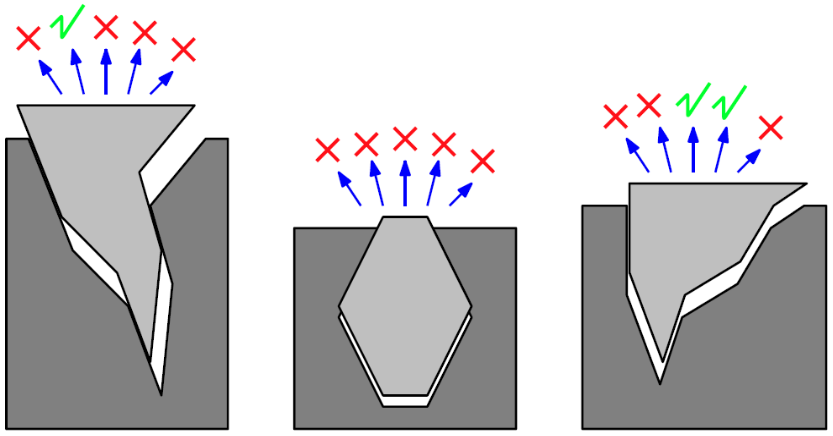
\includegraphics[width=0.6\linewidth]{afbeeldingen/gietvorm-voorbeeld}
		\label{fig:gietvorm-voorbeeld}
	\end{figure}
	
	De richting kan ook voorgesteld worden door pijlen in een bepaalde richting (geprojecteerd op $y=1$). Daar waar de richtingen overlappen, kan je dan naar boven trekken aan de vorm en zal je die in één keer eruit kunnen halen. Op dezefde manier kan die op een vlak geprojecteerd worden voor een 3d vorm. Hier hoort ook een lemma bij (dat ik zelf nog niet volledig snap)
	\begin{figure}[H]
		\centering
		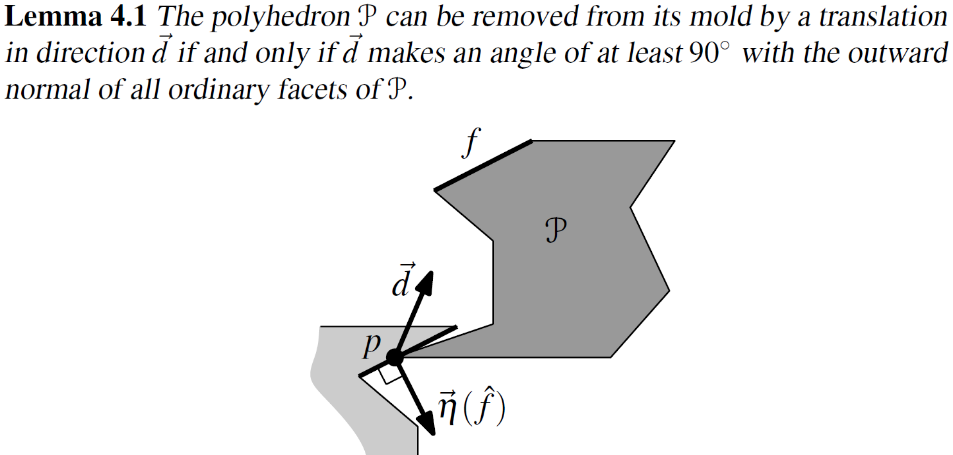
\includegraphics[width=0.7\linewidth]{afbeeldingen/gietvorm-lemm}
		\label{fig:gietvorm-lemma}
	\end{figure}
	
	Geldige richtingen in 3d kunnen voorgesteld worden door $n-1$ hafvlakken, met n het aantal vlakken van de vorm (waarbij -1 staat voor het bovenste vlak). De algemene vraag is dan: bereken de verzameling punten die beantwoorden aan alle constraints. Een interessante observatie is dat elk van die doorsnedes altijd een convexe vorm zal zijn. 
	
	
	\subsection{intersectie van halfvlakken}
	
	\begin{description}
		\item[Brute force]:\\
			Dit algoritme zal recursief berekenen wat de doorsnede is en gebruikt dan DCEL's om deze opnieuw te mergen. De pseudocode zal dit duidelijker maken: 
			\begin{figure}[H]
				\centering
				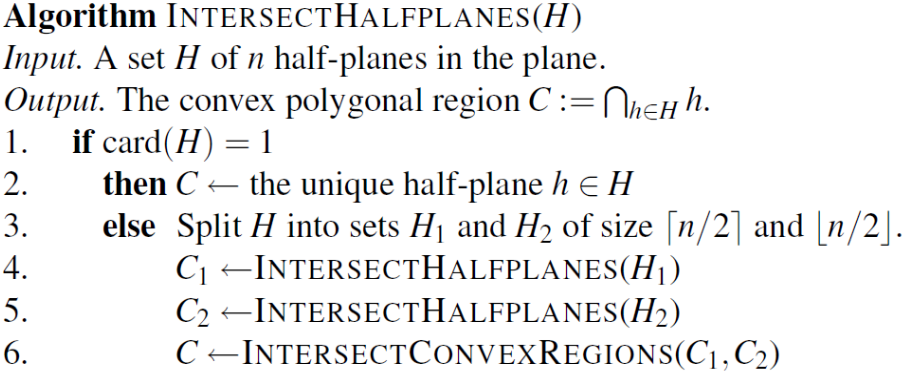
\includegraphics[width=0.8\linewidth]{afbeeldingen/intersectHalfPlanes}
				\label{fig:intersecthalfplanes}
			\end{figure}
			
		\item[Doorlooplijn]:\\
			Hier moet niet echt veel uitleg meer bij, het is gewoon een doorlooplijn die de linker- en rechterkant zal updaten met snijpunten als events.  
		\item[Incrementeel]:\\
			Voor het probleem van de gietvorm, is het genoeg één oplossing te kennen, en niet de volledige doorsneden. Alle halfvlakken kunnen gerepresenteerd worden door een vergelijking die groter moet zijn dan een bepaalde waarde, wat dus een rechte zal geven met een helft die wel mag gelden. We definiëren dan een functie f die afhankelijk is aan deze constraints en als we f maximaliseren, zullen we een bepaalde waarde hebben die deel is van de doorsnede. Het kan ook zijn dat we f blijven maximaliseren, maar dit zal uitkomen op een edge van de doorsneden, of zelfs tot in het oneindige voort zal gaan. 
			
			Dit algoritme is gelijkaardig aan een voor een een halfvlak toevoegen en veronderstellen dat de oplossing uniek is. Er zullen dus ook twee halfvlakken moeten geplaatst worden op de randen om de onbegrensde gevallen ook in rekening te brengen. Als bij het toevoegen van een halfvlak, de vertex nog steeds tot de doorsnede behoort: behouden we die vertex, anders moet er een nieuwe vertex gezocht worden. 
			\begin{figure}[H]
				\centering
				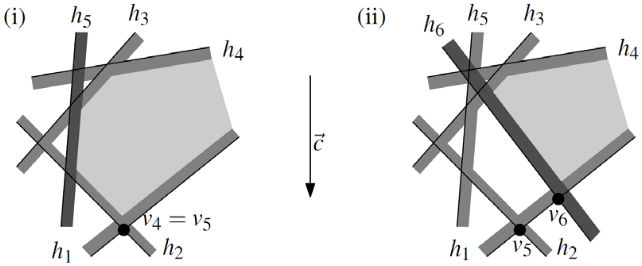
\includegraphics[width=0.7\linewidth]{afbeeldingen/gietvorm-incrementeel}
				\label{fig:gietvorm-incrementeel}
			\end{figure}
			
			De worst case is wanneer de vertex telkens opnieuw geplaatst moet worden, dan wordt de tijdscomplexiteit $O(n^2)$.
		\item[Random incrementeel]:\\
			Dit algoritme zal hetzelfe doen als het vorige, maar deze keer de halfvlakken willekeurig toevoegen. De kans bij een willekeurig halfvlak is $\frac{(i-2)}{i}$ de kans dat de laatste toevoeging een goedkope stap is. De tijdscomplexiteit zou dan $\sum_{i=1}^n O(i)\cdot\frac{2}{i} = O(n)$.
	\end{description}
	
	
	\subsection{kleinst omsluitende cirkel}
	Gegeven een set punten, wat is de kleinst omsluitende cirkel die je daarrond kan trekken. Een logische observatie is dat er een aantal punten op de cirkel zullen moeten liggen, anders is de cirkel niet minimaal. Specifieker zelfs: er zullen telkens minstens 3 punten op die cirkel liggen. Andere eigenschappen zijn: 1) De kleinst omsluitende cirkel is uniek, 2) indien een punt binnen in de cirkels weggehaald wordt, zal de cirkel zelf niet veranderen en 3) In dien een punt buiten de cirkel ligt, komt dat punt op de cirkel te liggen. 
	
	Dit probleem kan ook opgelost worden met een willekeurig incrementeel algoritme. Dit betekent dat er willekeurig telkens een punt zal toegevoegd worden en een voor een. Hierbij is het volgend lemmma belangrijk: 
	\begin{figure}[H]
		\centering
		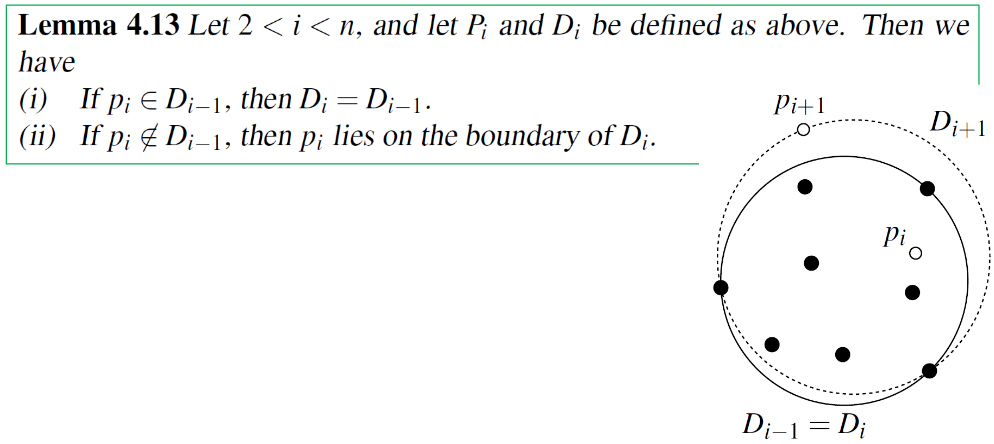
\includegraphics[width=0.8\linewidth]{afbeeldingen/cirkel-lemma}
		\label{fig:cirkel-lemma}
	\end{figure}
	
	De kleinste omsluitende cirkel voor n punten kan berekend worden met $O(n)$ tijdscomplexiteit. 
	
	
	\subsection{Gerandomiseerde incrementele algoritmen}
	Deze algoritmen zijn al hierboven besproken maar hier overlopen we de algemene eigenschappen nog eens. Bij deze algoritmen moet de test om na te gaan of de oplossing geldig is, snel zijn. Als de huidige oplossing herberekend moet worden, moet dit snel gebeuren. Het starten van het algoritme moet kunnen vanaf een kleine set voorwaarden. In de slides zijn er nog een aantal voorbeelden waarbij er gevraagd wordt of je die kan oplossen met RIC. 
	
	
	\section{Orthogonal Range searching, Kd-bomen}
	\subsection{Interval queries}
	We vragen ons af of we een algoritme kunnen maken om alle punten te bepalen die in een d-dimensionaal zoek-interval liggen. (Bijvoorbeeld: al de natuurlijkde getallen tussen 0 en 100)
	
	In 1D is dit: we willen een datastructuur vinden die ons gemakkelijk alle punten kan geven die tussen twee punten liggen. Het eerste waar we aan denken is dan een gebalanceerde binaire zoekboom: zoeken naar de kleinste waarde (of als deze er niet in ligt, de eerste waarde boven deze kleinste) en dan zoeken naar de grootste waarde van het interval. Bij het zoeken naar de kleinste en grootste waarde is het duidelijk dat er doorheen de zoekboom een pad overlopen zal worden. Alle 'subbomen' van die pad zullen deel zijn van de gegevensstructuur van het interval. 
	
	Het algoritme zal dus deze subbomen moeten bijhouden. In eerste instantie zal de 'split' node bijgehouden moeten worden. Zodra de split node is gevonden, kan de linkerboom gehandeld worden door elke rechtersubboom te rapporteren en het omgekeerde voor het rechterpad. Dit algoritme zal zorgen voor een geheugencomplexiteit $O(n)$. Het opbouwen van de zoekboom zal $O(n\log(n))$ complexiteit hebben en het zoeken zal 2 keer $O(\log(n))$ vragen om de kleinste en grootste waarde te zoeken. Daarna zal elk punt (k) in het interval ook nog overlopen worden, totale complexiteit van het zoeken van het interval is dus $O(\log(n) + k)$. 
	
	
	\subsection{Kd-boom}
	\begin{description}
		\item[Constructie]:\\
		Deze structuur is vooral om een interval in 2d te zoeken, er wordt dan afwisselend tussen x- en y-as afgewisseldn om de ruimte verder op te splitsen. De pseudocode om zo'n bomen op te stellen is hieronder te vinden: 
		\begin{figure}[H]
			\centering
			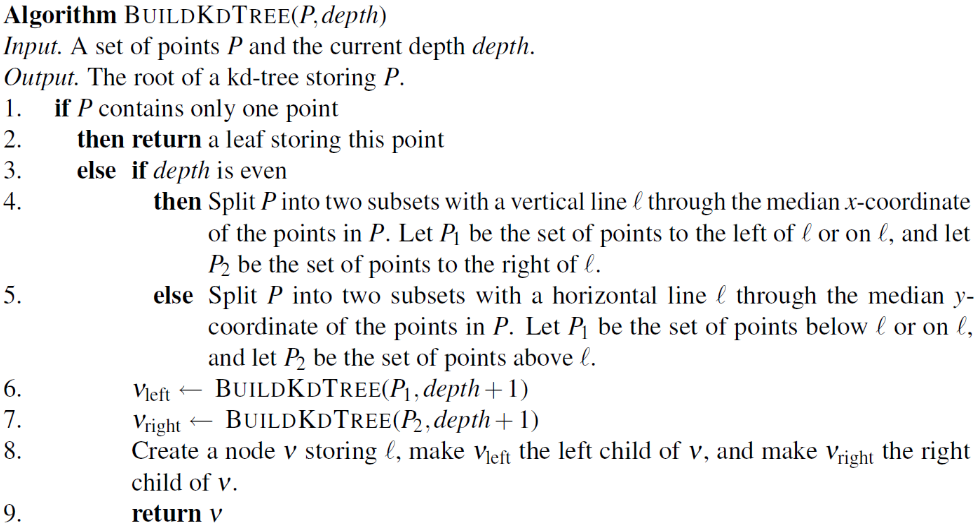
\includegraphics[width=0.7\linewidth]{afbeeldingen/kd-bomen/constructie}
			\label{fig:kd-constructie}
		\end{figure}
		Een kd-boom zal $O(n)$ aan geheugen nodig hebben en $O(n\log(n))$ aan tijdscomplexiteit. 
		\item[Zoeken]:\\
		Om te zoeken naar een interval, zal men de boom moeten aflopen. Elke knoop zal een extra grensniveau aanduiden en dus een kleinere regio definiëren. Hieronder volgen een goed visueel voorbeeld en de pseudocode voor dit algoritme. 
		\begin{figure}[h]
			\centering
			\subfigure[]{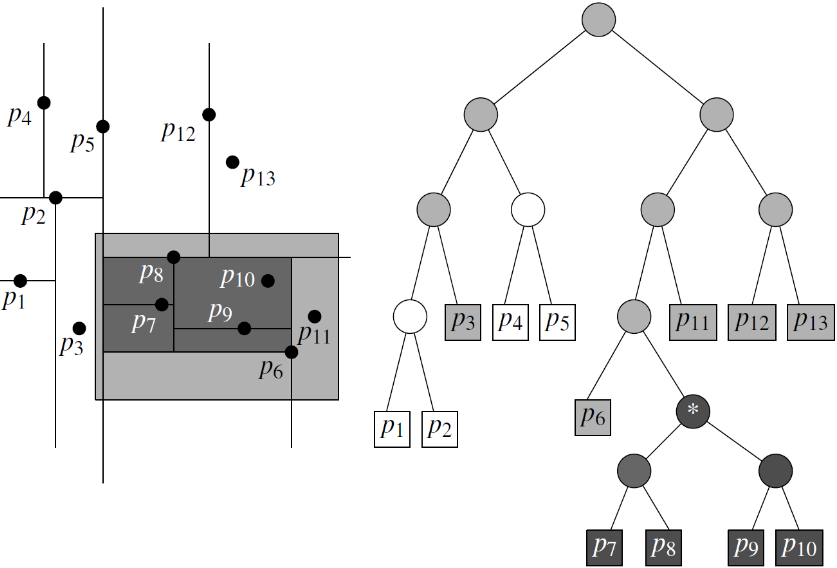
\includegraphics[width=0.40\textwidth]{afbeeldingen/kd-bomen/zoeken-voorbeeld}} 
			\subfigure[]{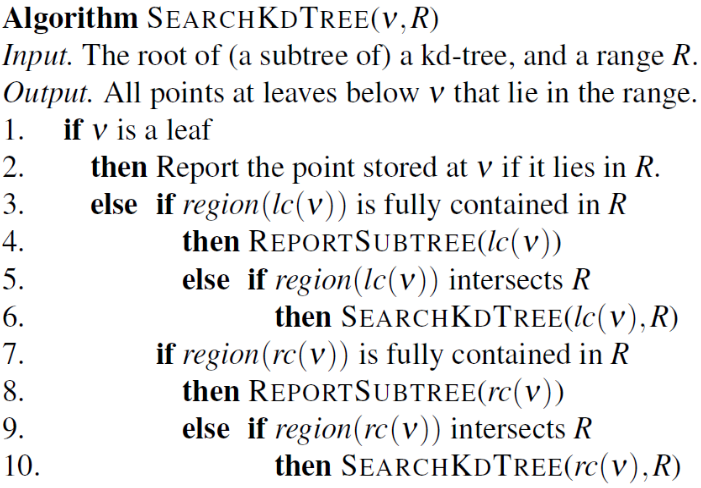
\includegraphics[width=0.40\textwidth]{afbeeldingen/kd-bomen/pseudocode}} 
			\label{fig:kd-zoeken}
		\end{figure}
		\item[efficiëntie]:\\
		Het rapporteren van de subbomen gebeurt in $O(k)$ met k het aantal punten dat teruggegeven moet worden als output. Het aantal knopen dat bezocht moet worden is $O(\sqrt{n})$. Deze expressie wordt gevonden door te kijken naar hoeveel regio's een horizontale lijn of een verticale lijn zou doorkruisen in zo'n regio in een kd-boom. Al deze doorsneden regio's vormen een boom met hoogte $\tfrac{1}{2}\log(n)$, aangezien we telkens twee grensniveaus moeten springen. Het totaal aantal regio's zal dan begrensd zijn door $2^{\frac{1}{2}\log(n)} = O(\sqrt{n})$. Zodra we beginnen aan hogere dimensies dan 2d, komen we aan een lineaire tijdscomplexiteit. 
	\end{description}
	
	
	\subsection{Range trees}
	Deze bomen zijn eigenlijk gelijk aan de kd-bomen, enkel dat ze snellere zoektijd willen bekomen ten koste van het geheugen. 
	
	Voor 1d houdt een range tree in: Vanaf een split node kunnen we opslaan wat de mogelijke eindknopen zijn van de zoekopdracht. 
	
	Voor 2d zal er een gebalanceerde boom zijn op basis van de x-coordinaat, in elke knoop is dan een nieuwe gebelanceerde boom op basis van de y-coordinaat. 
	
	Voor grotere dimensies voel je aan dat er dan per knoop nog extra dimensies zullen volgen. Elk punt zal maximaal 1 keer opgeslagen zijn in de boom $\rightarrow O(n)$ per niveau. Per punt zijn er dan $P(\log(n))$ niveaus  waarop het punt wordt opgeslagen. Het geheugen zal hier dus $O(n\log(n))$ zijn. De pseudocode voor het opbouwen en het zoeken zijn hieronder gegeven: 
	\begin{figure}[H]
		\centering
		\subfigure[]{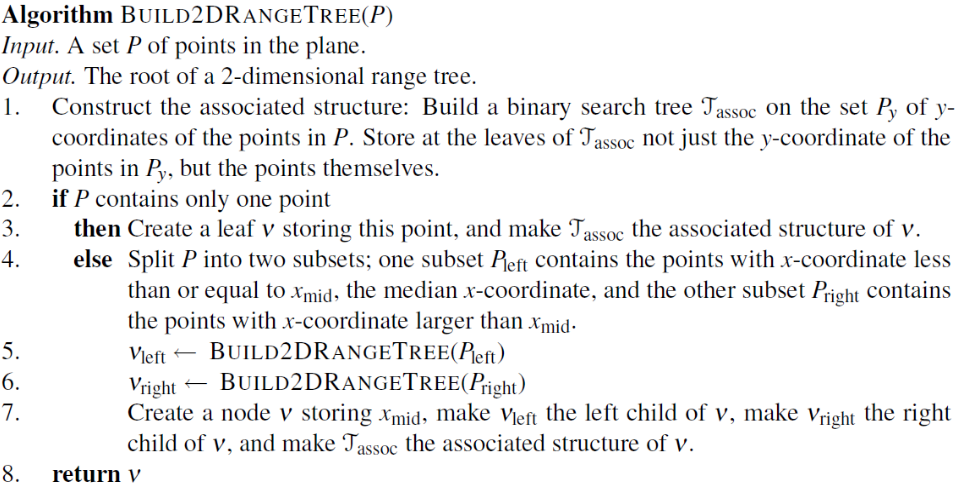
\includegraphics[width=0.49\textwidth]{afbeeldingen/kd-bomen/rangetree-build}} 
		\subfigure[]{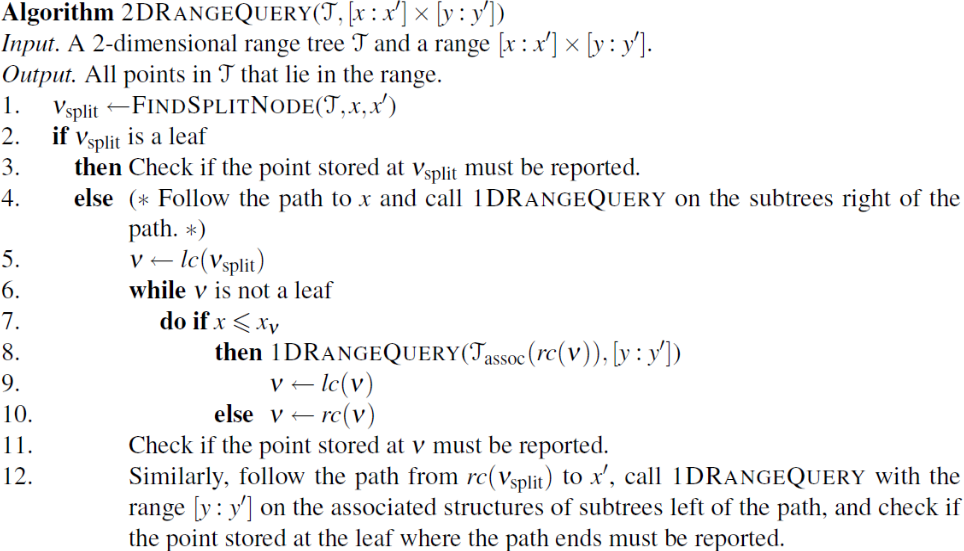
\includegraphics[width=0.49\textwidth]{afbeeldingen/kd-bomen/rangetree-zoeken}} 
		\label{fig:range-treees-pseudocode}
	\end{figure}

	De tijdscomplexiteit bij range zal inderdaad beteren, zoals hieronder te zien: 
	
	\begin{figure}[H]
		\centering
		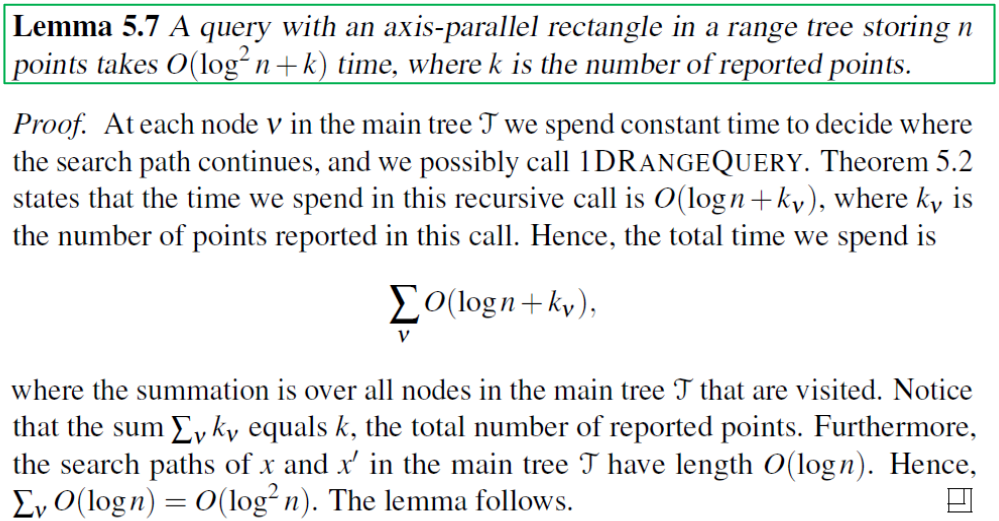
\includegraphics[width=0.7\linewidth]{afbeeldingen/kd-bomen/rangetrees-tijdscomplexiteit}
		\label{fig:rangetrees-tijdscomplexiteit}
	\end{figure}
	 
	
	
	\subsection{Typische examenvragen}
	\begin{itemize}
		\item \textbf{Wat is een kd-boom? Leg uit:}\\
		\item \textbf{Wat is de tijdscomplexiteit voor het opzoeken van alle punten binnen een (gegeven) 2D-interval in een tweedimensionale kd-boom?:}\\
		\item \textbf{Leg de idee uit van Range Trees:}\\
	\end{itemize}
	
	%TODO hier zit ik!
	\section{Puntlocatie}
	Deze les is gebaseerd op de vraag: ligt een punt in een gegeven veelhoek? 
	
	
	\subsection{Een aantal oplossingen}
	In dit deel worden een aantal oplossingen overlopen, allemaal heel simpel maar niet perse heel efficiënt. 
	\begin{itemize}
		\item We kunnen vanaf het punt kijken hoeveel snijpunten deze heeft met de veelhoek, als dit oneven is zal het punt in de veelhoek liggen. En probleem hiermee is wat al men hoekpunten tegenkomen? Dit is een edge case maar is wel heel relevant. 
		\item Een andere manier is de som te nemen van alle hoeken met alle hoekpunten van de veelhoek. Als de som van deze hoeken 0° is, dan is het punt buiten de veelhoek. Als de som 360° is, dan zit het punt wel in de veelhoek.
		\item Er is ook een manier om dit te bepalen met de kwadranten van een assenstelsel, waarbij er bijgeteld moet worden of niet bij het veranderen van een kwadrant. 
		\item Er kan een grid worden geplaatst over de veelhoek, afhankelijk van in wekl vierkantje het punt ligt weten we al op voorhand of het in de veelhoek zit of niet. In de vierkantjes kan ook een zijde van de veelhoek liggen, dan moeten er meer testen volgen. 
	\end{itemize}
	
	\subsection{Vlakverdeling}
	Een eerste aanpak tot het verdelen van de ruimte in verticale stroken die liggen op punten waar lijnen snijden. Het geheugencomplexiteit is dan $2n$, terwijl de tijdscomplexiteit om een punt te bepalen binnen een slab query $O(\log(n))$ is. Binnen zo een slab snijden er geen edges, deze kunnen dus gesorteerd worden op basis van y-coördinaat, elke slab heeft een $O(n)$ geheugen nodig. Het vinden van de locatie binnen de slab zal dus $O(\log(n))$ vragen. Het totale geheugen zal dus $O(n^2)$ vragen, wat niet ideaal is. 
	\\
	\\
	Een tweede aanpak is een \textit{trapezium map} opstellen van de vlakverdeling. Hier verbinden we elke vertex met de edge erboven en erronder. We veronderstellen hier dat elke vertex een verschillend x-coördinaat heeft en dat er een bounding box bestaat rond de vlakverdeling. De faces die zullen overblijven, zijn allemaal driekhoeken of trapezia. Deze trapezia zullen bepaald worden door: \textit{top, bottom, leftp, rightp}, top en bottom verwijzen naar edges en leftp en rightp verwijzen naar trapezia. Over deze trapezium map bestaat ook nog een lemma: 
	\begin{figure}[H]
		\centering
		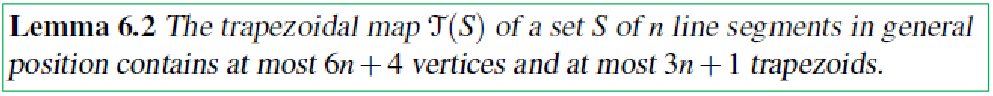
\includegraphics[width=0.9\linewidth]{afbeeldingen/trapezium-map/lemma}
		\label{fig:lemma}
	\end{figure}
	
	S zal bestaan uit $2n$ vertices, waarbij elke vertex 2 nieuwe vertices kan creëeren. De bounding box zelf bevat nog eens 4 vertices, wat een totaal geeft van $\rightarrow 4 + 2n + 2(2n) = 6n + 4$ vertices. Het links eindpunt van een segment kan een linkerzijde van 2 trapezia definiëren, een rechts eindpunt kan een linkerzijde van 1 trapezium definiëren. R definieerd del linkerzijde van 1 trapezium, diet komt neer op $3n + 1$ trapezia. Twee trapezia die aangrenzend zijn (dus een verticale lijn gemeenschappelijk) hebben altijd een top of bottom gemeenschappelijk. Elk lijnsegment zal in deze structuur verwijzen naar 2 eindpunten en de oorspronkelijke face die boven de edge ligt. Een trapezium kan dus via bottom te weten komen in welke face deze zit. 
	
	De effectieve gegevensstructuur die hiervoor kan gebruikt worden is een gerichte acyclische graaf (DAG). Elk blad is dan een trapezium, de x-knopen zijn de eindpunten van segmenten, deze verwijzen dan naar een lijnsegment (de y-knopen) die dan een boven en onder test hebben die verwijzen naar de trapezia. Het opstellen van deze graaf zal verlopen via een RIC (Randomized Incremental Constitution), zoals in de vorige les gezien. 
	Er zal dus telkens een nieuw lijnsegment worden toegevoegd en hier zal dus de trapezium map rond aangepast worden. Deze aanpasseingen gaan heel plaatselijk zijn, waardoor het RIC dus heel erg handig is. Het toevoegen van een lijnsegment zal twee stappen ondervinden:  
	\begin{enumerate}
		\item Als eerste overlopen we het nieuwe toegevoegde lijnstuk en duiden we alle trapezia waar die lijnstuk door ligt. Dit door telkens te zoeken naar bovenliggende lijnstukken, waarbij we het linkereindpunt zoeken en van daaruit kijken naar de trapezia. Hieronder volgt de pseudocode, voor een duidelijk visuele representatie: check de slides ;). 
		\begin{figure}[H]
			\centering
			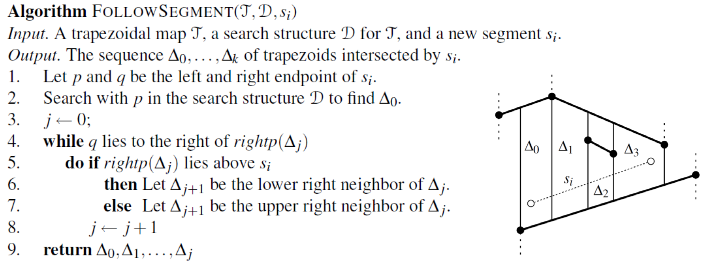
\includegraphics[width=0.7\linewidth]{afbeeldingen/trapezium-map/stap1-lijnstukken}
			\label{fig:stap1-lijnstukken}
		\end{figure}
		
		%TODO herbekijken in de les. 
		\item Als tweede zullen we de verticale verdeling updaten. In het algemene geval zal de graaf dan geüpdated moeten worden vanaf een bepaald niveau in de boom, en vraagt die niet ontzettend veel rekenwerk. 
	\end{enumerate}
	De tijdscomplexiteit van de eerste stap is het zoeken van k trapezia. $O(k)$. Dit is ook de comlexiteit van de tweede stap voor het aantal interne knopen en het aantal bladeren. 
	\\
	!! Examenvraag !!: Zo'n graaf kunnen opstellen voor een aantal lijnsegmenten, les opnieuw bekijken en snappen!!!
	
	De uiteindelijke trapezium zal niet afhangen van de RIC, maar de uiteindelijke graaf wel! Zo kan het zijn dat een graaf heel efficiënt is of net helemaal niet. Voor de analyse van de tijdscomplexiteit, kijken we naar de uitkomst want ik ben effe te moe om dit na te kijken en moet de les best herbekijken hiervoor. 
	\begin{figure}[H]
		\centering
		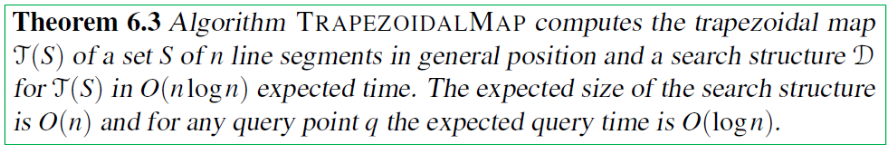
\includegraphics[width=0.9\linewidth]{afbeeldingen/trapezium-map/theorem}
		\label{fig:theorem}
	\end{figure}
	
	
	\subsection{Typische examenvragen}
	\begin{itemize}
		\item \textbf{Leg de pincipes uit van een trapezium-map:}\\
		\item \textbf{Leg het algoritme uit om een lijnsegment toe te voegen aan een bestaande trapezium-map:}\\
		\item \textbf{Op welke manieren kunnen we nagaan of een punt behoort tot het inwendige van een veelhoek?:}\\
	\end{itemize}
	
	
	\section{Voronoi Diagramma's}
	\subsection{Typische examenvragen}
	\begin{itemize}
		\item \textbf{Wat is het verband tussen het Voronoidiagramma van een verzameling punten, en de Delaunay triangulatie?:}\\
		\item \textbf{Leg het sweep-line algoritme van Fortune uit om een Voronoidiagramma te construeren:}\\
		\item \textbf{Bewijs eigenschap X van Voronoi-diagramma's. Welk belang heeft deze eigenschap voor de algoritmische constructie van Voronoi-diagramma's?:}\\
		\item \textbf{De Voronoi-veelhoek behorend bij een punt p dat behoort tot S is begrensd als en slechts als p behoort tot het inwendige van de convex omhullende van S. Bewijs deze eigenschap. Waar wordt deze eigenschap gebruikt, of waarom is ze nuttig?:}\\
		\item \textbf{Hoe bewijs je dat een Voronoi-diagram van een verzameling van N sites maximaal 2N-5 Voronoi-punten en maximaal 3N-6 Voronoi-zijden bezit? Waarom is het belangrijk dat het aantal Voronoi-zijden (slechts) O(N) is? Geef minstens één voorbeeld van het nut van deze eigenschap:}\\
		\item \textbf{(Gegeven een tekening met een aantal punten als Voronoi-sites en een positie van de doorlooplijn). Schets op bijhorende tekening het golffront voor de positie die de doorlooplijn reeds bereikt heeft, teken eveneens de Voronoi-punten en Voronoi-zijden die het algoritme van Fortune reeds bepaald heeft. Schrijf eventueel commentaar bij je tekening om één en ander te verduidelijken:}\\
		\item \textbf{Geef een voorbeeld waarbij de parabool behorende bij een Voronoi-site méér dan 1 segment bijdraagt aan het golffront (algoritme van Fortune):}\\
		\item \textbf{Geef een voorbeeld waarbij voor 6 Voronoi-sites, elk van de 6 sites door de doorlooplijn behandeld worden, vooraleer er een cirkel-event plaatsvindt. De sites moeten algemeen van aard zijn, ttz geen 3 sites op een lijn of 4 sites op een cirkel:}\\
	\end{itemize}
	
	
	\section{Delaunay Triangulatie}
	\subsection{Typische examenvragen}
	\begin{itemize}
		\item \textbf{Leg het verband uit tussen het Voronoi-diagramma van een puntenset en de Delaunay triangulatie van diezelfde puntenset:}\\
		\item \textbf{Op welke manier kan de Delaunay-triangulatie van een puntenset geconstrueerd worden?:}\\
		\item \textbf{Leg de equivalentie uit tussen de "cirkeleigenschappen" in zowel het Voronoi-diagramma als de Delaunay-triangulatie:}\\
		\item \textbf{Gegeven een set punten met bijhorende triangulatie. Is de getekende triangulatie een Delaunay-triangulatie? Waarom wel? Waarom niet? Welke eigenschappen kan je gebruiken om dit vast te stellen?:}\\
		\item \textbf{In een getekende Delaunay-triangulatie wordt een punt toegevoegd. Schets de resulterende Delaunay-tiangulatie:}\\
	\end{itemize}
	%Opmerking: vragen waarbij gevraagd wordt handmatig na te gaan of bepaalde eigenschappen gelden in een getekende Delaunay-triangulatie of Voronoi-diagramma zullen natuurlijk geen "milimeter-werk" zijn om iedereen op stang te jagen. Vaak zou je de cirkeleigenschappen met het blote oog moeten kunnen zien of gemakkelijk moeten kunnen afleiden met een eenvoudige construtie met een meetlat of passer ...
	
	
	\section{Béziercurven}
	\subsection{Typische examenvragen}
	\begin{itemize}
		\item \textbf{Gegeven een curve met enkele controlepunten met bijhorende curve: is dit (vermoedelijk) een Béziercurve? Waarom wel, waarom niet? Welke eigenschappen gebruik je om dit te achterhalen?:}\\
		\item \textbf{Gegeven enkele controlepunten: schets zo goed mogelijk (gebruik makende van eigenschappen van Béziercurven) de resulterende Bézier-curve:}\\
		\item \textbf{Wat zijn de belangrijkste eigenschappen van Béziercurven?:}\\
		\item \textbf{Leg uit: graadverhoging in Bézier-curven:}\\
		\item \textbf{Leg uit: Splitsing van Béziercurven:}\\
		\item \textbf{Leg uit hoe bij samengestelde Béziercurven C1- of C2-continuïteit voor de samengestelde curve bekomen wordt. Illustreer dit ook grafisch:}\\
		\item \textbf{Leg de ‘variatie-verminderingseigenschap’ van Bézier-curven uit. Waarom is deze belangrijk bij het ontwerp van curven?:}\\
		\item \textbf{Hoe vertaalt eigenschap X van Bernstein-veeltermen zich naar het gedrag van Bézier-curven?:}\\
	\end{itemize}
	
	
	\section{Binairy Space partitions}
	%The spiderman one
	\subsection{Typische examenvragen}
	\begin{itemize}
		\item \textbf{Wat is een Binary Space Partioning boom?:}\\
		\item \textbf{Bewijs dat een lage densiteits BSP boom O(n/k) bladknopen heeft:}\\
		\item \textbf{Wat is de bedoeling van de krimp-stap bij het opbouwen van een lage densiteits BSP boom?:}\\
		\item \textbf{Wat is het verband tussen een kd-boom en een BSP-boom?:}\\
		\item \textbf{Wat is de definitie van de dichtheid (density) van een set van objecten? Welk nut heeft de definitie van densiteit bij het opbouwen van een spatiale binaire zoekstructuur?:}\\
	\end{itemize}
	
	
	\section{Motion planning \& Visibility graphs}
\end{document}